%\documentclass{article}\usepackage[]{graphicx}\usepackage[]{color}
\documentclass[11pt,a4paper,oldfontcommands,openany]{memoir}
\usepackage{graphicx}
\usepackage[]{color}
%% maxwidth is the original width if it is less than linewidth
%% otherwise use linewidth (to make sure the graphics do not exceed the margin)
\makeatletter
\def\maxwidth{ %
  \ifdim\Gin@nat@width>\linewidth
    \linewidth
  \else
    \Gin@nat@width
  \fi
}
\makeatother

\definecolor{fgcolor}{rgb}{0.345, 0.345, 0.345}
\newcommand{\hlnum}[1]{\textcolor[rgb]{0.686,0.059,0.569}{#1}}%
\newcommand{\hlstr}[1]{\textcolor[rgb]{0.192,0.494,0.8}{#1}}%
\newcommand{\hlcom}[1]{\textcolor[rgb]{0.678,0.584,0.686}{\textit{#1}}}%
\newcommand{\hlopt}[1]{\textcolor[rgb]{0,0,0}{#1}}%
\newcommand{\hlstd}[1]{\textcolor[rgb]{0.345,0.345,0.345}{#1}}%
\newcommand{\hlkwa}[1]{\textcolor[rgb]{0.161,0.373,0.58}{\textbf{#1}}}%
\newcommand{\hlkwb}[1]{\textcolor[rgb]{0.69,0.353,0.396}{#1}}%
\newcommand{\hlkwc}[1]{\textcolor[rgb]{0.333,0.667,0.333}{#1}}%
\newcommand{\hlkwd}[1]{\textcolor[rgb]{0.737,0.353,0.396}{\textbf{#1}}}%

\usepackage{framed}
\makeatletter
\newenvironment{kframe}{%
 \def\at@end@of@kframe{}%
 \ifinner\ifhmode%
  \def\at@end@of@kframe{\end{minipage}}%
  \begin{minipage}{\columnwidth}%
 \fi\fi%
 \def\FrameCommand##1{\hskip\@totalleftmargin \hskip-\fboxsep
 \colorbox{shadecolor}{##1}\hskip-\fboxsep
     % There is no \\@totalrightmargin, so:
     \hskip-\linewidth \hskip-\@totalleftmargin \hskip\columnwidth}%
 \MakeFramed {\advance\hsize-\width
   \@totalleftmargin\z@ \linewidth\hsize
   \@setminipage}}%
 {\par\unskip\endMakeFramed%
 \at@end@of@kframe}
\makeatother

\definecolor{shadecolor}{rgb}{.97, .97, .97}
\definecolor{messagecolor}{rgb}{0, 0, 0}
\definecolor{warningcolor}{rgb}{1, 0, 1}
\definecolor{errorcolor}{rgb}{1, 0, 0}
\newenvironment{knitrout}{}{} % an empty environment to be redefined in TeX

\usepackage{alltt}
\setlength{\parindent}{0pt} % Remove indent at new paragraphs
\setcounter{secnumdepth}{4}  % Remove section numbering at certain depth # If zero, then no numbering of sections
\setcounter{tocdepth}{4} % Determines number of subsections that will have tabs
\usepackage{tabu}
\usepackage[round,sort]{natbib}
\usepackage{fixltx2e}
%\usepackage{graphicx}	% For external pictures
\usepackage{float}
\usepackage{subfig}	% Add subfigures within figures
\usepackage{verbatim}
\usepackage[colorlinks=true,linkcolor=blue,citecolor=blue,urlcolor=blue]{hyperref}
\usepackage{amssymb,amsbsy,amsmath}
\usepackage{epsfig}
\usepackage[left=3cm,top=3cm,bottom=3.5cm,right=3cm]{geometry} % For easy document margins
%\usepackage{fancyhdr} % For customization of header/footer
\usepackage{adjustbox}
\usepackage{framed}
\usepackage{enumitem}
\usepackage{caption}
\numberwithin{equation}{section} % Equation numbers relative to sections
\usepackage[dvipsnames]{xcolor}

%%%%% NEW ADDED FROM THESIS.TEX %%%%% 
\usepackage[utf8]{inputenc}
\usepackage[T1]{fontenc}
\usepackage{microtype}
%\usepackage[dvips]{graphicx}
%\usepackage{times} %clash
%%%%%%%%%%%%%%%%%%%%%%%%%%%%%%%%%%%%%%%% 
\newcommand{\code}[1]{{\texttt{#1}}}
\newcommand{\pkg}[1]{{\texttt{#1}}}
\newcommand{\class}[1]{{\textit{#1}}}
\newcommand{\R}{{\normalfont\textsf{R }}{}}
\IfFileExists{upquote.sty}{\usepackage{upquote}}{}


\begin{document}

\sloppy

%%%%%%%%%%%%%%%%%%%%% TITLE PAGE %%%%%%%%%%%%%%%%%%%%%

{
\centering
~\vspace{\fill}

\vspace{2.5cm}

{\LARGE Thesis Proposal}

\vspace{1cm}

{\LARGE\textbf{Visualization methods for genealogical and RNA-sequencing datasets}}

\vspace{1cm}

{\LARGE Lindsay Rutter}

\vspace{4cm}

{\LARGE Program of Study Committee:}

\vspace{1cm}

{\LARGE Dianne Cook, Major Professor}

\vspace{.25cm}

{\LARGE Amy Toth, Major Professor}

\vspace{.25cm}

{\LARGE Heike Hofmann}

\vspace{.25cm}

{\LARGE Daniel Nettleton}

\vspace{.25cm}

{\LARGE James Reecy}

\vspace{2.5cm}

{\centerline{\large May 16, 2016}}
}

\clearpage
%\cleardoublepage

%%% CHAPTER'S STYLE
\chapterstyle{bianchi}
\setsecheadstyle{\Large\bfseries\sffamily\raggedright}
\setsubsecheadstyle{\large\bfseries\sffamily\raggedright}
\setsubsubsecheadstyle{\bfseries\sffamily\raggedright}
%%%%%%%%%%%%%%%%%%%%%%%%%%%%%%%%%%%%

\tableofcontents

\setlength{\parskip}{10pt} % Inter-paragraph spacing

%%% ADDED FROM THESIS.TEX %%%%%%%%%
\OnehalfSpacing

\chapter{Introduction}

\section{Background to data visualization}

Blah blah blah Blah blah blah Blah blah blah Blah blah blah Blah blah blah Blah blah blah Blah blah blah Blah blah blah Blah blah blah Blah blah blah Blah blah blah Blah blah blah Blah blah blah Blah blah blah Blah blah blah Blah blah blah Blah blah blah.

\section{Problems to be addressed}

Blah blah blah Blah blah blah Blah blah blah Blah blah blah Blah blah blah Blah blah blah Blah blah blah Blah blah blah Blah blah blah Blah blah blah Blah blah blah Blah blah blah Blah blah blah Blah blah blah Blah blah blah Blah blah blah Blah blah blah.

\section{Overview of thesis research}
\label{sec:helpSection}

Blah blah blah Blah blah blah Blah blah blah Blah blah blah Blah blah blah Blah blah blah Blah blah blah Blah blah blah Blah blah blah Blah blah blah Blah blah blah Blah blah blah Blah blah blah Blah blah blah Blah blah blah Blah blah blah Blah blah blah.

\chapter{Visualization methods for genealogical datasets}
\label{sec:ggenealogy}

\section{Abstract}

In this chapter, we introduce \pkg{ggenealogy} (\cite{ggen}), a developing \proglang{R} software package that provides tools for searching through genealogical data, generating basic statistics on their graphical structures using parent and child connections, and displaying the results. The package allows users to draw the genealogy in relation to variables related to the nodes, and to determine and display the shortest path distances between the nodes. Production of pairwise distance matrices and genealogical diagrams constrained on generation are also available in the visualization toolkit. We are testing the tools on a dataset with milestone cultivars of soybean varieties (\cite{soybean}) as well as on a web-based database of the academic genealogy of mathematicians (\cite{mgp}). 
The software package has been available on the Comprehensive \proglang{R} Archive Network since March 2015. 

\chapter{Stock syntax}
\section{Database structure}

Blah blah blah Blah blah blah Blah blah blah Blah blah blah Blah blah blah Blah blah blah Blah blah blah Blah blah blah Blah blah blah Blah blah blah Blah blah blah Blah blah blah Blah blah blah Blah blah blah Blah blah blah Blah blah blah Blah blah blah. As an example, the learning outcomes for \texttt{Topic 03} are provided in List \hyperref[sec:lo]{1} below.
As seen in Figure \ref{fig:overviewFigure}.

\begin{center}
\captionsetup{width=\textwidth}
\fbox{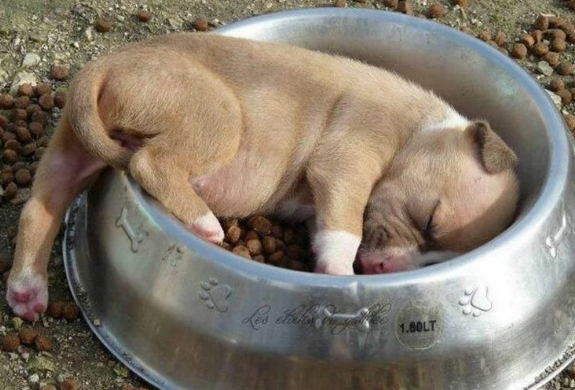
\includegraphics[width=\textwidth]{stock.png}}
\captionof{figure}{Caption blah blah blah blah blah blah blah blah blah blah blah blah blah blah blah blah blah blah blah blah blah}
\label{fig:overviewFigure}
\end{center}

Now, we will run the \hyperref[sec:helpSection]{REFER TO SECTION }.

%%%%%%%%%%%%%%%%%%%%%% TABLE EXAMPLE %%%%%%%%%%%%%%%%%%%%%%
%%%%%%%%%%%%%%%%%%%%%%%%%%%%%%%%%%%%%%%%%%%%%%%%%%%%%%%%%%%
\begin{center}
\captionof{table}{Topic numbers and descriptions}
\label{tab:topics}
\begin{tabular} { | l | l | }
\hline \textbf{Number} & \textbf{Description} \\
\hline
01 & Data \\
\hline
02  & Descriptive Statistics for a Single Categorical Variable \\
\hline
03 & Descriptive Statistics for a Single Quantitative Variable \\
\hline
\end{tabular}
\end{center}
%%%%%%%%%%%%%%%%%%%%%%%%%%%%%%%%%%%%%%%%%%%%%%%%%%%%%%%%%%%

%%%%%%%%%%%% ENUMERATION - A/B/C EXAMPLE %%%%%%%%%%%%%%%%%%
%%%%%%%%%%%%%%%%%%%%%%%%%%%%%%%%%%%%%%%%%%%%%%%%%%%%%%%%%%%
\centerline{List 1: Learning outcomes for Topic 03}
\vspace{-2mm}
\begin{framed}
\begin{enumerate}[label=\Alph*.]
\label{sec:lo}
\item Use standardizing to determine how many standard deviations an observation is away from the mean value.
\item Use z-scores to compare observations for different quantitative variables.
\item Explain how standardizing affects the shape, center, and variability of the distribution of a quantitative variable.
\end{enumerate}
\end{framed}
%%%%%%%%%%%%%%%%%%%%%%%%%%%%%%%%%%%%%%%%%%%%%%%%%%%%%%%%%%%

%%%%%%%%%%%%%%%%%%%%%%% COLOR TEXT %%%%%%%%%%%%%%%%%%%%%%%%
%%%%%%%%%%%%%%%%%%%%%%%%%%%%%%%%%%%%%%%%%%%%%%%%%%%%%%%%%%%
\begin{framed}
Example question title: \textbf{\textcolor{Red}{T16}.\textcolor{YellowOrange}{A}.\textcolor{YellowGreen}{A}.\textcolor{Green}{04-1}.\textcolor{blue}{1}.\textcolor{RedViolet}{MC}.\textcolor{VioletRed}{1}}
\end{framed}
%%%%%%%%%%%%%%%%%%%%%%%%%%%%%%%%%%%%%%%%%%%%%%%%%%%%%%%%%%%

%%%%%%%%%%%%%%%%%%%%% EXAMPLE CODE %%%%%%%%%%%%%%%%%%%%%%%%
%%%%%%%%%%%%%%%%%%%%%%%%%%%%%%%%%%%%%%%%%%%%%%%%%%%%%%%%%%%
The absolute pathway to the \texttt{extdata} directory on your local computer can be determined by typing the following command into the \textbf{\textsf{R}} console: \\

\begin{knitrout}
\definecolor{shadecolor}{rgb}{0.969, 0.969, 0.969}\color{fgcolor}\begin{kframe}
\begin{alltt}
\hlkwd{system.file}\hlstd{(}\hlstr{"inst/extdata/"}\hlstd{,} \hlkwc{package} \hlstd{=} \hlstr{"ePort"}\hlstd{)}
\end{alltt}
\end{kframe}
\end{knitrout}

\begin{knitrout}
\definecolor{shadecolor}{rgb}{0.969, 0.969, 0.969}\color{fgcolor}\begin{kframe}
\begin{alltt}
\hlstd{keyHTM} \hlkwb{=} \hlkwd{system.file}\hlstd{(}\hlstr{"inst/extdata/KeyFiles/Topic06.Questions.htm"}\hlstd{,} \hlkwc{package} \hlstd{=}
  \hlstr{"ePort"}\hlstd{)}

\hlkwd{refineKey}\hlstd{(keyHTM)}

\hlstd{keyPath} \hlkwb{=} \hlkwd{gsub}\hlstd{(}\hlstr{"htm$"}\hlstd{,} \hlstr{"txt"}\hlstd{, keyHTM)}

\hlstd{dataPath} \hlkwb{=} \hlkwd{system.file}\hlstd{(}\hlstr{"inst/extdata/DataFiles/Topic06/Topic06.A.csv"}\hlstd{,} \hlkwc{package} \hlstd{=}
  \hlstr{"ePort"}\hlstd{)}

\hlkwd{rewriteData}\hlstd{(dataPath)}

\hlstd{loPath} \hlkwb{=} \hlkwd{system.file}\hlstd{(}\hlstr{"inst/extdata/LOFiles/Topic06.Outcomes.txt"}\hlstd{,} \hlkwc{package} \hlstd{=} \hlstr{"ePort"}\hlstd{)}

\hlstd{outPath} \hlkwb{=} \hlkwd{system.file}\hlstd{(}\hlstr{"inst/extdata/OutputFiles"}\hlstd{,} \hlkwc{package} \hlstd{=} \hlstr{"ePort"}\hlstd{)}

\hlkwd{makeReport}\hlstd{(}\hlkwc{keyFile} \hlstd{= keyPath,} \hlkwc{dataFile} \hlstd{= dataPath,} \hlkwc{loFile} \hlstd{= loPath,} \hlkwc{outFile} \hlstd{=}
  \hlstd{outPath)}
\end{alltt}
\end{kframe}
\end{knitrout}

\begin{knitrout}
\definecolor{shadecolor}{rgb}{0.969, 0.969, 0.969}\color{fgcolor}\begin{kframe}
\begin{alltt}
\hlstd{merged} \hlkwb{=} \hlkwd{subsetData}\hlstd{(mergedData, dataTable)}
\hlkwd{makeReport}\hlstd{(}\hlkwc{outFile} \hlstd{= outPath,} \hlkwc{unit} \hlstd{=} \hlnum{2}\hlstd{,} \hlkwc{reportType} \hlstd{=} \hlstr{"crossSecUnit"}\hlstd{,} \hlkwc{className} \hlstd{=}
  \hlstr{"Eng444"}\hlstd{,} \hlkwc{repeatLowScore} \hlstd{=} \hlnum{70}\hlstd{)}
\end{alltt}
\end{kframe}
\end{knitrout}
%%%%%%%%%%%%%%%%%%%%%%%%%%%%%%%%%%%%%%%%%%%%%%%%%%%%%%%%%%%

%%%%%%%%%%%%%%%%%% LIST (BULLETS) %%%%%%%%%%%%%%%%%%%%%%%%
%%%%%%%%%%%%%%%%%%%%%%%%%%%%%%%%%%%%%%%%%%%%%%%%%%%%%%%%%%%
\begin{framed}
\begin{itemize}
\vspace{-3mm}
\item One topic for one section - short version (``secTopicShort")
\item One topic for one section - long version (``secTopicLong")
\item One topic comparing multiple sections - short version (``crossSecTopicShort")
\item One topic comparing multiple sections - long version (``crossSecTopicLong")
\item One unit (group of topics) for one section (``secUnit")
\item One unit (group of topics) comparing multiple sections (``crossSecUnit")
\end{itemize}
\end{framed}
%%%%%%%%%%%%%%%%%%%%%%%%%%%%%%%%%%%%%%%%%%%%%%%%%%%%%%%%%%%

\bibliography{myThesis}
\bibliographystyle{plain}

\end{document}
